\documentclass{article}

\usepackage[final]{neurips_2020}
\usepackage[utf8]{inputenc} % allow utf-8 input
\usepackage[T1]{fontenc}    % use 8-bit T1 fonts
\usepackage{hyperref}       % hyperlinks
\usepackage[pdftex]{graphicx}
\usepackage{url}            % simple URL typesetting
\usepackage{booktabs}       % professional-quality tables
\usepackage{amsfonts}       % blackboard math symbols
\usepackage{nicefrac}       % compact symbols for 1/2, etc.
\usepackage{microtype}      % microtypography

\title{Atomic Force Microscopy}

\author{
Umur Can Kaya\\
5410770\\
\texttt{umurcan.kaya@gmail.com}\\
\And
Rohit Sharma\\
5442717\\
\texttt{rohis97@zedat.fu-berlin.de}\\
}

\begin{document}
\maketitle

\begin{abstract}
The aim of this experiment is to become familiar with the working principles and operation of the atomic force microscope , which we use to determine the surface topography of two samples (Au on HOPG and Au on Si(111)), to calculate the relative work function between Au and HOPG, and to determine the tip geometry of the microscope.
\end{abstract}
\section{Introduction}

Scanning probe microscopy is a branch of microscopy that allows for the imaging of surfaces at atomic resolutions by using a physical probe that scans the sample. The first ever successful realization of scanning microscopy was the scanning tunnelling microscope.

The scanning tunneling microscope (STM), invented in 1981, was the first instrument to allow real space imaging of surfaces at atomic resolutions. It exploits the quantum mechanical phenomenon of tunneling between the tip and the sample to map the surface of conductive samples. STM's inherent limitation of being able to image only conductive samples led to the development of atomic force microscope.

The advantages of AFM, invented in 1986, over STM includes being able to image surfaces of insulating materials and liquids, measurement of atomic forces between the sample and the tip, and sample manipulation. AFM includes a tip that is placed on the free end of a cantilever and the sample is scanned under this tip as shown in figure \ref{fig:schematic_afm}. At close enough distances the tip and the sample interact through atomic forces and direct or indirect measurement of these forces give information about the surface topography of the sample.

\begin{figure}[h!]
\centering
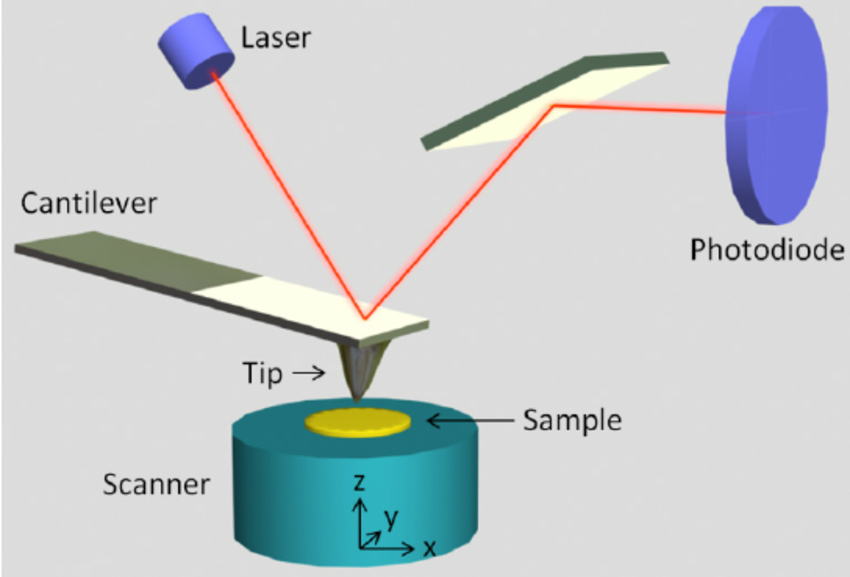
\includegraphics[width=0.6\linewidth]{LAB/AFM/Schematic-AFM.png}
\caption{Schematic illustration of the principles of AFM. The scanner controls the horizontal ($x$ and $y$) and vertical ($z$) movement of the sample. [2]}
\label{fig:schematic_afm}
\end{figure}

\subsection{Imaging modes}
AFM can be operated in two different modes: contact mode where the tip is essentially dragged over the surface of the sample with a repulsive surface-tip interaction, and non-contact mode where the tip is not in contact with the surface but oscillated above it.

In contact AFM the tip is held at a distance of a few angstroms to the surface, this is in the regime where the net force between the tip and the sample is positive and therefore repulsive, causing a soft physical contact. Then the sample is scanned under the tip resulting with the deflection of the cantilever. The deflection data can be translated to topography image by using one of the two scanning modes explained in section \ref{sec:scanning_modes}.

In non-contact AFM, the cantilever oscillates near its resonance frequency due to an oscillating driving force while being held at a distance from the surface. In this mode, information about the topography of the surface is not obtained directly from the deflection of the cantilever but from the changes in the frequency and amplitude of the oscillation. The cantilever is modeled as a linear elastic that obeys Hooke's Law and therefore its resonance frequency is directly proportional with the square root of the spring constant $\omega_0 = \sqrt{k/m}$. Resonance frequency is shifted in the presence of tip-sample forces which is a function of distance. This shift can be translated to topography data again by using one of the two scanning modes explained in section \ref{sec:scanning_modes}. Non-contact AFM has a major advantage over contact AFM, it preserves the sample surface and AFM tip since the forces acting on both are weaker, this allows for higher quality samples after imaging, and extended usability of the tip.

\subsection{Scanning modes}
\label{sec:scanning_modes}
There are two scanning modes in atomic force microscopy based on the parameter that is kept constant during he scanning process. In constant height mode the distance between the tip and the sample is kept constant while the deflection of the cantilever is directly interpreted as topographic data. 

On the other hand, in the constant force mode it is the force between tip and sample which it is maintained constant with a feedback circuit which takes the input of the deflection of the cantilever information and adjusts the height of the &z& scanner where the sample is placed. It will e precisely this height which will be read as the topographic data. Even if the speed of the constant force mode is limited by the time response of the feedback circuit it is normally preferred as an operation mode because it allow us to control the force exerted on the sample. These two scanning modes can be used in contact and non-contact Atomic Force Microscopy.

\subsection{Involved atomic forces}
There are several kinds of forces at play between the tip and the sample.The short-range chemical force (repulsive and attractive forces) is described by the Lennard-Jones potential:
\begin{equation}
    U_{chem} = 4 \epsilon[(\frac{\sigma_0}{r})^{12} - (\frac{\sigma_0}{r})^{6}
\end{equation}
where $\epsilon$ is the strength of the minimal potential and $\sigma_{0}$ is the distance of the zero-potential. The forces become repulsive when distances are less than $\sigma_{0}$ and become attractive when greater than the same. In practice, Van der Waal forces are used here as
\begin{equation}
    F_{vdW}= \frac{HR}{6(d^{6})}
\end{equation}
where H is the Hamaker constant, R is the radius of the tip and d is the
tip-sample distance. \\
Another force which have to remember in this case is the the force due to the potential difference between the sample and tip namely the electrostatic force. It is given by
\begin{equation}
    F_{elec}=1/2 \frac{\delta C}{\delta Z}V^{2}_{eff}
\end{equation}
where C is the capacitance of the tip-sample capacitor and $V_{eff}$ is the effective voltage. The tip is acted on by the sum of all these forces.
\begin{equation}
    F_{tot} = F_{vdW} + F_{electrostatic} + F_{chem}
\end{equation}
Cantilever oscillation is approximated by equation of motion for a damped harmonic oscillator with forced oscillations.
 \begin{equation}
     m\ddot{z} + \gamma \dot{z} + kz = F_{0}\cos(\omega t) + F_{tot}
 \end{equation}
where z is the tip-sample distance, $\gamma$ is the damping of the oscillation, $k$ is the spring constant of the cantilever and $F_{0}\cos(\omega t)$ is the force from the oscillation made by the piezoelectric element
Resonance frequency of the oscillation is \begin{equation}
    \omega_{0} = \sqrt{\frac{k}{m}}
\end{equation}
The interaction between tip and sample can now be included by a change in the spring constant of the cantilever 
\begin{equation}
    k_{eff} = K \frac{-\delta F_{tot}}{\delta Z} 
\end{equation}
The new resonance frequency should be shifted with respect to the free resonance. 

\subsection{Tip geometry}

\section{Experimental setup}
A typical AFM consists of a cantilever with a small tip at the free end, a laser, a 4-quadrant photodiode and a scanner as seen in figure. AFM measurements are made by a Nanotec microscope. Sample is mounted on the piezo at the center. AFM head has to be positioned appropriately at the center of the sample. The laser should be reflecting off the mid point of the canteliver. One must make sure that the photodiode alignment is so configured that the photodiode obtains maximum reflected laser beam.
\section{Tasks}

\subsection{Experimental preparation}

\subsection{Surface topography of Au on HOPG}

\subsection{Relative work function between Au and HOPG}

\subsection{Tip geometry}

\subsection{Surface topography of Au on Si}

\section{Discussion}


\section*{References}

[1] 

[2] Nanomechanics of Amyloid Materials Studied by Atomic Force Microscopy - Scientific Figure on ResearchGate. Available from: https://www.researchgate.net/figure/Schematic-illustration-of-the-principles-of-AFM-The-scanner-is-composed-of-three-piezo_fig1_221927184 [accessed 13 Dec, 2021]

\end{document}
